%% ----------------------------------------------------------------
%% ProjectManagement.tex
%% ---------------------------------------------------------------- 
\chapter{Project Management} 
\label{Chapter: Project Management}

\begin{preamble}
Due to the large and complex nature of the project care was taken to ensure the group's time and effort was managed effectively. This chapter gives details regarding how the group formed as well as the general positions within the team each member took. Information about the groups working procedure is given along with details of how the group communicated within itself and with project stakeholders.
\end{preamble}

\section{Formation} 
\label{Section:Formation}

Although as a whole the group had never worked together in the past, some existing close working relationships existed due to previous group coursework. As such it was easy to form the group and begin producing impressive results.

\subsection{Skills Audit} 
\label{Section:Skills Audit}

Many of the strengths and weaknesses of the group members were clear from previous work, but a skills audit was undertaken to ensure that the group as a whole was competent to complete both the coursework and the project without fault.

To begin with a requirement analysis was performed to determine exactly what skills were needed. These split into three very clear general subsections: project management and leadership, from the perspective of both the coursework and the project; technical; and communication. 

Next an audit of each teams members skills were performed, the results of which can be found in \autoref{Chapter:Skills Audit Results}. From these an analysis of the groups total skills was determined and the groups weaknesses could be found.

\section{Task and Work Management} 
\label{Section:Task and Work Management}

This project was run using a Scrum project management approach. This involved having weekly sprints where each person completed a number of tasks, either alone or collaborating with others. Planning meetings were held at the start of each sprint where the issues in the backlog were discussed. They were prioritised and given a point value which related to how much time and effort the issue would take to resolve. The highest priority issues were then assigned. Each person had a maximum capacity of points for each week. Additionally retrospectives were held just prior to the planning meetings to discuss the previous sprints and the way in which the project management was being carried out.

This structure meant that planning and the monitoring of the project happened formally on a sprint by sprint basis. But throughout the project we were careful to adapt when needed, and not be too constrained by the Scrum model. At points in the project where progress presentations had to be created, practised and presented we ran ``mini-sprints'' both for the presentation, and work to be completed in the remainder of the week.

\subsection{Roles and Responsibilities}

Throughout the project all members took on a number of project roles. These roles were both technical and management based, with care being taken to allow for flexibility between and within roles. Roles and responsibilities were assigned dynamically with members volunteering when they felt they were the best fit.

\begin{description}
  \item[Christopher Baines] \hfill \\
  	Christopher took a technical lead, focusing on architectural design and component interaction. Much of his work was in-depth and complex in nature. His particular focuses were the webworker videogular-questions and analytics server.
  \item[Samuel Bennett] \hfill \\
  	Samuel took a leadership role early in the project. He spent much of his time removing technical blockers for other members and acting as a central hub, keeping all members abreast with the work of others. Technically he used his previous AngularJS knowledge to begin the code bases for the project, as well as working closely with Christopher Baines in determining the general architectural design. Much of his technical work was done on videogular-questions, both the front end and the webworker.
  \item[Harry Cutts] \hfill \\
  	Harry took a technical role. He focused his attention on ensuring the project work was being completed to a good standard, he took a lead in determining our code conventions. Harry produced and released videogular-cuepoints, taking time to ensure it was opensourced properly.  He also took on part of the role of scrum master, ensuring the group conformed to the agile process.
  \item[Christopher Hewett] \hfill \\
  	Christopher took both a technical and leadership role. His technical work was not focused on any particular project but rather completing large amounts of tasks on all projects. Once of his earlier key themes was completing work on the styling of all frontends. In the last few weeks prior to Christmas Christopher took on a leadership role in ensuring everything was completed on time.
  \item[Maria Lynch] \hfill \\
  	Maria's technical contributions focused on the initial design and implementation of the authoring tool, and the design and implementation of the heatmaps plugin. Maria took responsibility for organising the coursework deliverables. She edited much of the reports and managed their production. UI design and accessibility was another of her key focusses.
\end{description}

Generally the group felt that all members completed similar amounts of work over the course of the project, as well as sharing equal responsibility.

\subsection{Management Problems}

Throughout the project a number of management problems were encountered and worked around.

Sam's bereavement - Group worked around it and chewett took over
Group modifying agile methods
group adjusting amount of points
groups other courseworks

\subsection{Collaboration and Issue Management}
To allow for collaborative work a GitHub organisation\footnote{\url{https://github.com/soton-ecs-2014-gdp-12/}} was used. This acted as our central source code repository for not only all directly related work, but also work on presentations and reports. Separate repositories for each area of the project are located here for ease of access. Using GitHub made it easier to interact with other open source projects, and all our pull requests and releases were directed from here. 

GitHub also provided an issue management system on a repository by repository basis. This allowed us to track conversations around different bugs and enhancements as the project progressed.
The group used \url{http://www.waffle.io} to manage the issues backlog from a project wide perspective as this would interface directly with GitHub.

\subsection{Statistics}

Due to the tracked nature of the project's work it is easy to produce retrospective statistical analysis.

By tracking commits within the GitHub organisation (over 1000) one can determine when the the week work was generally completed. This data is visualised in \autoref{fig:punchard}. The group generally completed most of their work as it would have been done in an industrial setting, during standard office hours with extra work being doing late into the evenings and on weekends.

%http://tex.stackexchange.com/questions/86114/github-like-punchcard-with-the-help-of-pgfplots
\begin{figure}
  \makebox[\textwidth][c]{
\begin{tikzpicture}                                             %1
        \begin{axis}[                                               %2
                grid=major,                                         %3
                point meta=explicit,
                xmin=-1,
                xmax=24,
                xlabel=Hours,                                       %7
                scatter/@pre marker code/.code={
                    \pgfmathparse{                                  %12
                        sqrt(\pgfplotspointmetatransformed)/50*12}   %13
                    \def\markopts{                                  %14
                        mark=*,                                     %15
                        color=black,                     %16
                        fill=black,                      %17
                        mark size=\pgfmathresult}                   %18
                    \expandafter\scope\expandafter[\markopts]},
                scatter/@post marker code/.code={
                    \endscope},
                symbolic y coords={Sun,Sat,Fri,Thu,Wed,Tue,Mon},
                xtick={0,...,23},
                x=0.55cm,
                y=0.9cm]
            \addplot[only marks,scatter]
                table[x index=0, y index=1, meta index=2] {punchcard.dat};
        \end{axis}
\end{tikzpicture}
  }%
  \caption{A punchard diagram showing the frequency of commits at different hours of the day. The area is proportional to the number of commits.}
  \label{fig:punchard}
\end{figure}

By tracking closed issues on a week by week basis it is possible to determine when work was completed throughout the project. Although issues are of different sizes, over the sample of 100s of issues a general grasp can be achieved. A graph of this can be seen in \autoref{fig:tasksweek}. It shows that generally the same amount of work was completed in every week. Week 8's deficiency can be explained by the larger nature of the issues as well as the second progress presentation and other coursework needing to be completed that week. Weeks 12 to 17  being lower is explained by first the christmas break and then examinations. 

%Sam has the code to generate this form the Github API
\begin{figure}
\centering
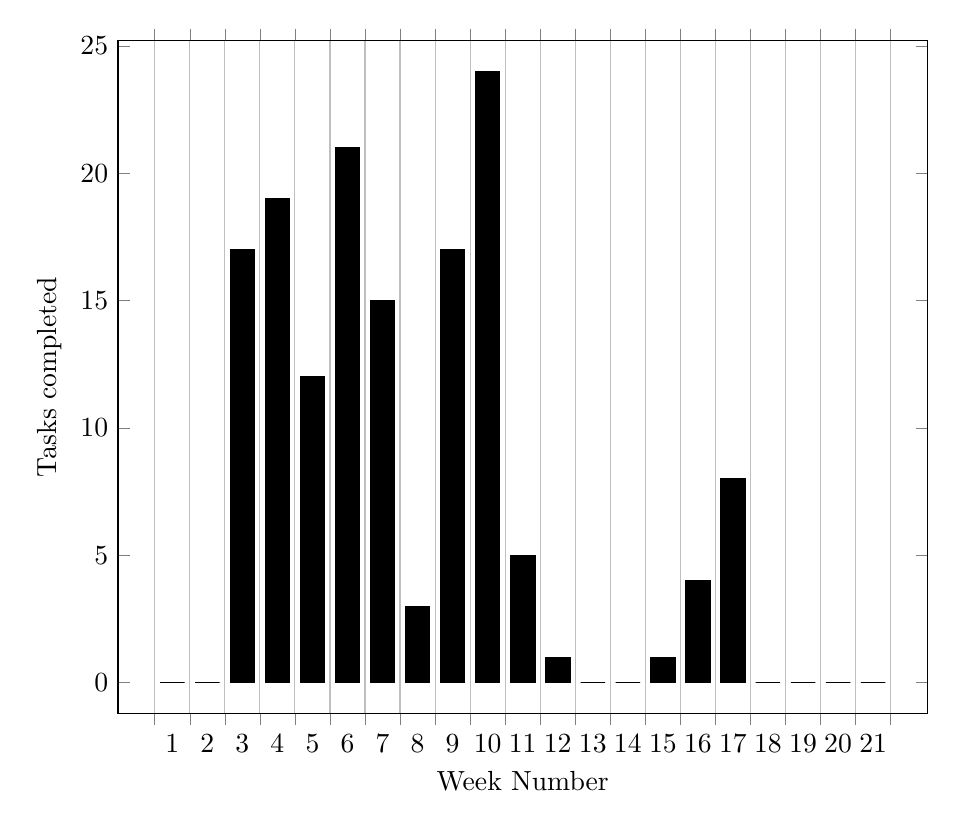
\begin{tikzpicture}
\begin{axis}[
	scale=1.5,
	ylabel={Tasks completed},
	xlabel= {Week Number},
	enlargelimits=0.05,
	ybar interval=0.7,
]
\addplot[black,fill=black]
	coordinates {(1, 0) (2, 0) (3, 17) (4, 19) (5, 12) (6, 21) (7, 15) (8, 3) (9, 17) (10, 24) (11, 5) (12, 1) (13, 0) (14, 0) (15, 1) (16, 4) (17, 8) (18, 0) (19, 0) (20, 0) (21, 0) (22, 0) };
\end{axis}
\end{tikzpicture}
  \caption{A bar chart of the number of Github issues being closed in each week of the project.}
  \label{fig:tasksweek}
\end{figure}

\section{Client Management} 
\label{Section:Client Management}

The project had a reasonably large number of stakeholders that needed to be managed and kept informed. Each stakeholder required different levels of communication via different methods.

The most important stakeholder was the client, Professor Mike Wald. Weekly meeting were organised, minutes of which can be found in \autoref{Chapter:Minutes of Meetings}, and emails were used for urgent issues. 

Final project sign-off to check for client satisfaction was gathered using a deliverable report. It was delivered prior to the sign-off meeting and then discussed. It can be found in \autoref{Chapter:Deliverable Report}.

Another important stakeholder was Yunjia Li. He attend the weekly meetings as much as possible so as to ensure his future interests in the framework were protected. He was also contactable via email when needed.

2fdev, the Videogular development team, were communicated with via Gitter\footnote{\url{https://gitter.im/2fdevs/videogular}}, an online chat system added onto GitHub. They had an ongoing interest with the framework due to its role of advertising the Videogular project.  There advice and code proved invaluable throughout the project.

Shameem Bajar provided valuable user feedback. She both came to meetings as well as communicated with the group via email.
